\documentclass{standalone}
\usepackage{tikz}
\usepackage{xcolor}
\usetikzlibrary{patterns, positioning}
\usetikzlibrary{shapes.misc}
\usepackage[outline]{contour}
\contourlength{1.5pt} 


\begin{document}
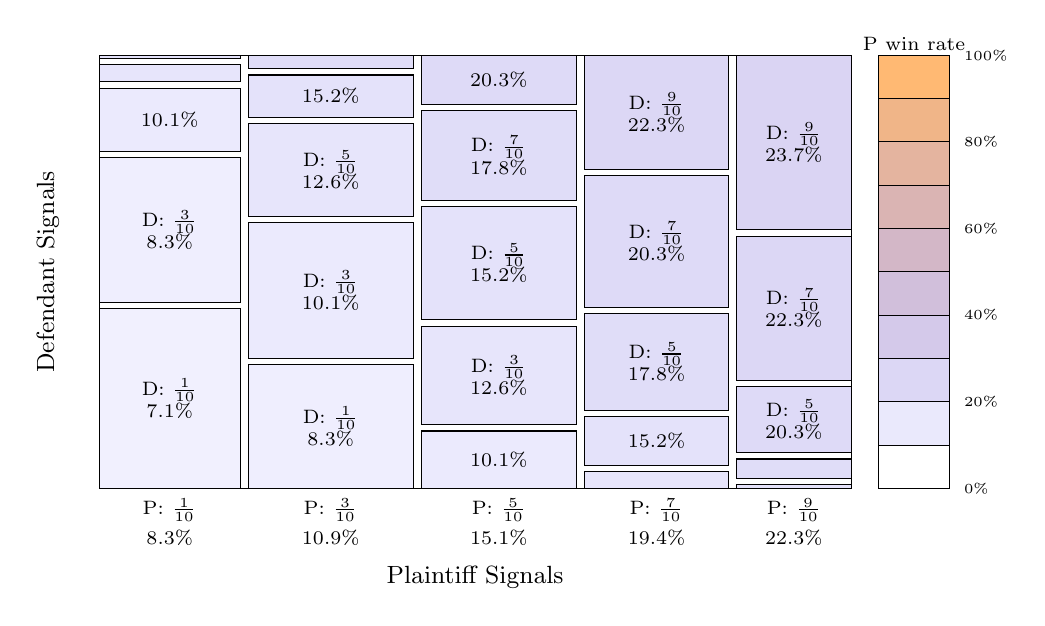
\begin{tikzpicture}
\newcommand{\DFractionOffset}{0.4}
\newcommand{\AxisLabelYAdjust}{-0.235}
\draw[draw=black] (0.6,2) rectangle (10.15,7.5);
\draw[fill=blue!93!orange!7!white!86!white, draw=black] (0.6,2) rectangle (2.3926,4.2834);
\draw (1.496288732173734, 3.1417165302978134) node[font=\scriptsize, text=black, align=center] {D: $\frac{1}{10}$\\ 7.1\%};
\draw[fill=blue!92!orange!8!white!85!white, draw=black] (0.6,4.3634) rectangle (2.3926,6.2009);
\draw (1.496288732173734, 5.282186278821729) node[font=\scriptsize, text=black, align=center] {D: $\frac{3}{10}$\\ 8.3\%};
\draw[fill=blue!90!orange!10!white!85!white, draw=black] (0.6,6.2809) rectangle (2.3926,7.0836);
\draw (1.496288732173734, 6.682259327461665) node[font=\scriptsize, text=black, align=center] {10.1\%};
\draw[fill=blue!87!orange!13!white!84!white, draw=black] (0.6,7.1636) rectangle (2.3926,7.3807);
\draw[fill=blue!85!orange!15!white!83!white, draw=black] (0.6,7.4607) rectangle (2.3926,7.5);
\draw (1.496288732173734, 1.6) node[anchor=north, font=\scriptsize, text=black] {8.3\%};
\draw (1.496288732173734, {1.6 + \DFractionOffset}) node[anchor=north, font=\scriptsize, text=black] {P: $\frac{1}{10}$};
\draw[fill=blue!92!orange!8!white!85!white, draw=black] (2.4926,2) rectangle (4.5893,3.571);
\draw (3.5409349891004416, 2.785484090781383) node[font=\scriptsize, text=black, align=center] {D: $\frac{1}{10}$\\ 8.3\%};
\draw[fill=blue!90!orange!10!white!85!white, draw=black] (2.4926,3.651) rectangle (4.5893,5.3763);
\draw (3.5409349891004416, 4.51363445897159) node[font=\scriptsize, text=black, align=center] {D: $\frac{3}{10}$\\ 10.1\%};
\draw[fill=blue!87!orange!13!white!84!white, draw=black] (2.4926,5.4563) rectangle (4.5893,6.6319);
\draw (3.5409349891004416, 6.044121135879945) node[font=\scriptsize, text=black, align=center] {D: $\frac{5}{10}$\\ 12.6\%};
\draw[fill=blue!85!orange!15!white!83!white, draw=black] (2.4926,6.7119) rectangle (4.5893,7.2504);
\draw (3.5409349891004416, 6.981164010775201) node[font=\scriptsize, text=black, align=center] {15.2\%};
\draw[fill=blue!82!orange!18!white!82!white, draw=black] (2.4926,7.3304) rectangle (4.5893,7.5);
\draw (3.5409349891004416, 1.6) node[anchor=north, font=\scriptsize, text=black] {10.9\%};
\draw (3.5409349891004416, {1.6 + \DFractionOffset}) node[anchor=north, font=\scriptsize, text=black] {P: $\frac{3}{10}$};
\draw[fill=blue!90!orange!10!white!85!white, draw=black] (4.6893,2) rectangle (6.6616,2.7295);
\draw (5.6754650057421365, 2.364741913768956) node[font=\scriptsize, text=black, align=center] {10.1\%};
\draw[fill=blue!87!orange!13!white!84!white, draw=black] (4.6893,2.8095) rectangle (6.6616,4.0593);
\draw (5.6754650057421365, 3.4343703905755767) node[font=\scriptsize, text=black, align=center] {D: $\frac{3}{10}$\\ 12.6\%};
\draw[fill=blue!85!orange!15!white!83!white, draw=black] (4.6893,4.1393) rectangle (6.6616,5.5788);
\draw (5.6754650057421365, 4.859032173217972) node[font=\scriptsize, text=black, align=center] {D: $\frac{5}{10}$\\ 15.2\%};
\draw[fill=blue!82!orange!18!white!82!white, draw=black] (4.6893,5.6588) rectangle (6.6616,6.801);
\draw (5.6754650057421365, 6.2299222786229365) node[font=\scriptsize, text=black, align=center] {D: $\frac{7}{10}$\\ 17.8\%};
\draw[fill=blue!80!orange!20!white!81!white, draw=black] (4.6893,6.881) rectangle (6.6616,7.5);
\draw (5.6754650057421365, 7.190518582211586) node[font=\scriptsize, text=black, align=center] {20.3\%};
\draw (5.6754650057421365, 1.6) node[anchor=north, font=\scriptsize, text=black] {15.1\%};
\draw (5.6754650057421365, {1.6 + \DFractionOffset}) node[anchor=north, font=\scriptsize, text=black] {P: $\frac{5}{10}$};
\draw[fill=blue!87!orange!13!white!84!white, draw=black] (6.7616,2) rectangle (8.5961,2.2121);
\draw[fill=blue!85!orange!15!white!83!white, draw=black] (6.7616,2.2921) rectangle (8.5961,2.9075);
\draw (7.678868102618596, 2.59982563775195) node[font=\scriptsize, text=black, align=center] {15.2\%};
\draw[fill=blue!82!orange!18!white!82!white, draw=black] (6.7616,2.9875) rectangle (8.5961,4.2156);
\draw (7.678868102618596, 3.601577695959154) node[font=\scriptsize, text=black, align=center] {D: $\frac{5}{10}$\\ 17.8\%};
\draw[fill=blue!80!orange!20!white!81!white, draw=black] (6.7616,4.2956) rectangle (8.5961,5.9689);
\draw (7.678868102618596, 5.132259498252166) node[font=\scriptsize, text=black, align=center] {D: $\frac{7}{10}$\\ 20.3\%};
\draw[fill=blue!78!orange!22!white!81!white, draw=black] (6.7616,6.0489) rectangle (8.5961,7.5);
\draw (7.678868102618596, 6.774449827470952) node[font=\scriptsize, text=black, align=center] {D: $\frac{9}{10}$\\ 22.3\%};
\draw (7.678868102618596, 1.6) node[anchor=north, font=\scriptsize, text=black] {19.4\%};
\draw (7.678868102618596, {1.6 + \DFractionOffset}) node[anchor=north, font=\scriptsize, text=black] {P: $\frac{7}{10}$};
\draw[fill=blue!85!orange!15!white!83!white, draw=black] (8.6961,2) rectangle (10.15,2.0485);
\draw[fill=blue!82!orange!18!white!82!white, draw=black] (8.6961,2.1285) rectangle (10.15,2.3731);
\draw[fill=blue!80!orange!20!white!81!white, draw=black] (8.6961,2.4531) rectangle (10.15,3.2928);
\draw (9.423049353803169, 2.8729592667792874) node[font=\scriptsize, text=black, align=center] {D: $\frac{5}{10}$\\ 20.3\%};
\draw[fill=blue!78!orange!22!white!81!white, draw=black] (8.6961,3.3728) rectangle (10.15,5.2037);
\draw (9.423049353803169, 4.2882615871635) node[font=\scriptsize, text=black, align=center] {D: $\frac{7}{10}$\\ 22.3\%};
\draw[fill=blue!76!orange!24!white!80!white, draw=black] (8.6961,5.2837) rectangle (10.15,7.5);
\draw (9.423049353803169, 6.391862571646354) node[font=\scriptsize, text=black, align=center] {D: $\frac{9}{10}$\\ 23.7\%};
\draw (9.423049353803169, 1.6) node[anchor=north, font=\scriptsize, text=black] {22.3\%};
\draw (9.423049353803169, {1.6 + \DFractionOffset}) node[anchor=north, font=\scriptsize, text=black] {P: $\frac{9}{10}$};
\node[font=\small, text=black] at (5.375, {1.1 + \AxisLabelYAdjust}) {Plaintiff Signals};
\node[font=\small, text=black, rotate=90] at (-0.050000000000000044, 4.75) {Defendant Signals};
\draw[draw=black] (10.5,2) rectangle (11.4,7.5);
\draw (10.95, 7.65) node[font=\scriptsize, text=black] {P win rate};
\draw[fill=blue!100!orange!0!white!88!white, draw=black] (10.5,2) rectangle (11.4,2.55);
\draw[fill=blue!89!orange!11!white!84!white, draw=black] (10.5,2.55) rectangle (11.4,3.1);
\draw[fill=blue!78!orange!22!white!81!white, draw=black] (10.5,3.1) rectangle (11.4,3.65);
\draw[fill=blue!67!orange!33!white!77!white, draw=black] (10.5,3.65) rectangle (11.4,4.2);
\draw[fill=blue!56!orange!44!white!73!white, draw=black] (10.5,4.2) rectangle (11.4,4.75);
\draw[fill=blue!44!orange!56!white!70!white, draw=black] (10.5,4.75) rectangle (11.4,5.3);
\draw[fill=blue!33!orange!67!white!66!white, draw=black] (10.5,5.3) rectangle (11.4,5.85);
\draw[fill=blue!22!orange!78!white!62!white, draw=black] (10.5,5.85) rectangle (11.4,6.4);
\draw[fill=blue!11!orange!89!white!59!white, draw=black] (10.5,6.4) rectangle (11.4,6.95);
\draw[fill=blue!0!orange!100!white!55!white, draw=black] (10.5,6.95) rectangle (11.4,7.5);
\draw (11.46, 2) node[anchor=west, font=\tiny, text=black] {0\%};
\draw (11.46, 3.1) node[anchor=west, font=\tiny, text=black] {20\%};
\draw (11.46, 4.2) node[anchor=west, font=\tiny, text=black] {40\%};
\draw (11.46, 5.3) node[anchor=west, font=\tiny, text=black] {60\%};
\draw (11.46, 6.4) node[anchor=west, font=\tiny, text=black] {80\%};
\draw (11.46, 7.5) node[anchor=west, font=\tiny, text=black] {100\%};


\end{tikzpicture}
\end{document}